%-----------------------------------------------------------------------
% 中国科学: 信息科学 中文模板, 请用 CCT-LaTeX 编译
% http://scis.scichina.com
%-----------------------------------------------------------------------

\documentclass{SCIS2020cn}
%%%%%%%%%%%%%%%%%%%%%%%%%%%%%%%%%%%%%%%%%%%%%%%%%%%%%%%
%%% 作者附加的定义
%%% 常用环境已经加载好, 不需要重复加载
%%%%%%%%%%%%%%%%%%%%%%%%%%%%%%%%%%%%%%%%%%%%%%%%%%%%%%%
\usepackage{listings}

%%%%%%%%%%%%%%%%%%%%%%%%%%%%%%%%%%%%%%%%%%%%%%%%%%%%%%%
%%% 开始
%%%%%%%%%%%%%%%%%%%%%%%%%%%%%%%%%%%%%%%%%%%%%%%%%%%%%%%
\begin{document}

%%%%%%%%%%%%%%%%%%%%%%%%%%%%%%%%%%%%%%%%%%%%%%%%%%%%%%%
%%% 作者不需要修改此处信息
\ArticleType{学生基础训练}
%\SpecialTopic{}
%\Luntan{中国科学院学部\quad 科学与技术前沿论坛}
\Year{2021}
\Vol{50}
\No{1}
\BeginPage{1}
\DOI{}
\ReceiveDate{}
\ReviseDate{}
\AcceptDate{}
\OnlineDate{}
%%%%%%%%%%%%%%%%%%%%%%%%%%%%%%%%%%%%%%%%%%%%%%%%%%%%%%%

\title{对数几率回归}{对数几率回归}

\entitle{Title}{Title for citation}

\author[1]{袁满杰}{{yuanmanjie@foxmail.com}}


\address[1]{南京大学, 南京 210023}


\AuthorMark{第一作者等}


\abstract{本文对拟牛顿法的基本思想和理论进行了回顾。}


\keywords{拟牛顿法, 机器学习}

\maketitle

\section{理论回顾}

\subsection{牛顿法 }
牛顿法的思想是对于一个待优化的函数$f(x)$,其使用二阶泰勒展开作为其近似,并以泰勒展开的极值点近似原函数的极值点优化目标函数,并一轮轮迭代上述优化过程。相比于梯度下降算法,其使用了二阶信息,因此优化速度更快。
\\以$x$为一维时为例,对于最优化问题:
\begin{equation*}
    \min_x f(x)
\end{equation*}
下一轮$x_{t+1}$使用在上一轮$x_t$处的二阶泰勒展开近似:
\begin{equation*}
    f(x_{t+1})=f(x_t)+\nabla f(x_t)\Delta x_t+\frac{1}{2}\Delta x_t^T \nabla^2f(x_t) \Delta x_t
\end{equation*}
令$H_t=\nabla^2f(x_t)$代表其Hessian阵。 则选择最优化了该泰勒展开的点作为下一轮$x_{t+1}$,令其偏导等于0:
\begin{equation*}
    {\nabla f(x_{t+1})}=\nabla f(x_t)+H_t\Delta x_t =0
\end{equation*}
可解得:
\begin{equation*}
    \Delta x_t =-H_t^{-1}\nabla f(x_t)
\end{equation*}
因此,牛顿法的迭代更新公式为:
\begin{equation}
    x_{t+1}=x_t-H_t^{-1}\nabla f(x_t)
\end{equation}

\section{拟牛顿法}
\subsection{算法思想}
由于Hessian阵往往计算麻烦,且需要求矩阵的逆,计算量大,复杂度高,反而会导致算法效率下降。因此我们考虑一种迭代式的、不需要直接计算逆矩阵和Hessian矩阵,但又能足够逼近真实Hessian阵的方法。用形式化表述,我们旨在通过迭代的方式寻找一个$B_k$,每轮迭代公式为$B_{t+1}=B{t}+\Delta$,且原函数的梯度近似变为了;
\begin{equation*}
{\nabla f(x_{t+1})}=\nabla f(x_t)+B_{t+1}\Delta x_t 
\end{equation*}
为保证目标函数能有效地被优化,我们应确保上述梯度的近似在$x_t$和$x_{t+1}$两处均与真实梯度相等。当$\Delta x_t=0$时,其在$x_t$处自然相等,因此我们只需让其在$x_{t+1}$处也与真实梯度相等,也即:
\begin{equation*}
    \nabla f(x_t)+B_{t+1}\Delta x_t =\nabla f(x_{t+1})
\end{equation*}
令$s_t=\Delta x_t=x_{t+1}-x_t$,$y_t=\nabla f(x_{t+1})-\nabla f(x_t)$,则整理可得:
\begin{equation}
    B_{t+1}s_t=y_t
\end{equation}
上式即称为拟牛顿条件,不同的拟牛顿法则是用不同的迭代方法来找到满足上述条件的Hessian阵近似$B_t$。拟牛顿法可以表述为以下的优化问题:
\begin{eqnarray}
    B_{t+1}=\arg\min_B ||B-B_t||\\
    s.t.\ B=B^T, Bs_t=y_t
\end{eqnarray}

不同的拟牛顿法可以视为是选用不同范数下的解。

\subsection{DFP法 }
以上述矩阵最优化问题的思路,当取范数为加权的F范数(如\ref{eq1}所示),且以如\ref{eq2}所示的平均Hessian阵的逆时,也即$W=G_k^{-1}$,之前所示的最优化问题的解便是DFP法。
\begin{equation}
    \label{eq1}
    ||A||_W=||W^{1/2}AW^{1/2}||_F=||C||_F=\sqrt{\sum_{i=0}^n\sum_{j=0}^nc^2_{ij}}
\end{equation}
\begin{equation}
    \label{eq2}
    G_k=\int_0^1 \nabla^2 f(x_t+\tau \Delta x_t)d\tau
\end{equation}

但上述优化方法数学性比较强,较为晦涩,这里我们另外考虑一种通过构造的方式,来对DFP方法进行推导。回到我们的目标,我们旨在找出一个对称矩阵,使其满足拟牛顿条件。考虑到牛顿法最终的迭代公式中需要Hessian阵的逆矩阵,不妨我们直接估计$D\approx H^{-1}$,使其满足拟牛顿条件如\ref{eq3}.
\begin{equation}
    \label{eq3}
    \Delta x_t=D_{t+1}\Delta g_t
\end{equation}
而因为我们采用迭代的方法来求$D_{t+1}\approx H^{-1}$,将$D_{t+1}-D_t=\Delta D_t$带入\ref{eq3}即可得:
\begin{equation}
    \label{eq4}
    \Delta D_{t}\Delta g_t=\Delta x_t -D_t\Delta g_t
\end{equation}
而每轮迭代中我们可利用的信息除了上一轮的$D_t$之外,只有$\Delta x_t$和$\Delta g_t$.因此,出于方便计算的考虑,也出于和\ref{eq4}形式一致而易解出参数的考虑,不妨我们假设更新公式是$\Delta x_t$和$D_t\Delta g_t$的一个线性组合如\ref{eq5}.
\begin{equation}
    \label{eq5}
    \Delta D_t=\Delta x_t q_t^T-D_t\Delta g_t w_t^T
\end{equation}
对照\ref{eq4}和\ref{eq5}可得:
\begin{equation}
    \label{eq6}
    q_t^T\Delta g_t=w^T_t\Delta g^t=I_n
\end{equation}
除此之外,为了保证$D_t$一定是对称矩阵,最直接的方法就是直接令$q_t$和$w_t$分别与$\Delta x_t$和$D_t\Delta g_t$平行,也即做如下\ref{eq7}的假设。
\begin{eqnarray}
    \label{eq7}
    q_t=\alpha_t \Delta x_t\\
    w_t=\beta_t D_t\Delta g_t
\end{eqnarray}
联立以上三式可解得:
\begin{eqnarray}
    \alpha_t=\frac{1}{\Delta g_t^T\Delta x_t}
    \beta_t=\frac{1}{\Delta g_t^TD_t\Delta g_t}
\end{eqnarray}
带回\ref{eq5}可得到最终$D_t$的更新公式:
\begin{equation}
    \Delta D_t=\frac{\Delta x_t\Delta x_t^T}{\Delta g_t^T\Delta x_t}-\frac{D_t\Delta g_t\Delta g_t^TD_t}{\Delta g_t^TD_t\Delta g_t}
\end{equation}
不过,因为拟牛顿法在一边更新$D_t$的过程中一边优化原目标函数,因此不同于牛顿法,拟牛顿法只取$-D_tg_t$为搜索方向,之后还需在该方向上做一维搜索确定步长,也即需做如下的更新:
\begin{eqnarray}
    d_t=-D_tg_t\\
    \lambda_t=\arg\min_\lambda f(x_t+\lambda d_t)\\
    x_{t+1}=x_t+\lambda_t d_t
\end{eqnarray}

\subsection{BFGS法 }
BFGS法与DFP法类似,只不过其不直接拟合$H^{-1}$,而是去拟合Hessian阵$H$本身,而后其使用Sherman-Morrison公式来以直接更新的方式求逆矩阵。\\
对于BFGS法,只需要将DFP法中的$\Delta x_t$和$\Delta g_t$交换,便可得到如下的拟牛顿条件和更新公式:
\begin{eqnarray}
    \Delta g_t=B_{t+1}\Delta x_t\\
    \Delta B_t=\frac{\Delta g_t\Delta g_t^T}{\Delta x_t^T\Delta g_t}-\frac{B_t\Delta x_t\Delta x_t^TB_t}{\Delta x_t^TB_t\Delta x_t}
\end{eqnarray}
但在更新步长时仍需用到$B^{-1}_t$,因此其使用Sherman-Morrison公式,对于任意非奇异方阵$A$和n维向量$u,v$,若$1+v^TA^{-1}u\neq 0$,则:
\begin{equation}
    (A+uv^T)^{-1}=A^{-1}-\frac{(A^{-1}u)(v^TA^{-1})}{1+v^TA^{-1}u}
\end{equation}
也即对于在$A$上的修改后得到的新方阵$A+uv^T$的逆,我们可以直接通过$A^{-1}$和$u,v$计算得到,而不需要重新计算新方阵的逆。因此最终BFGS法直接对$B^{-1}$迭代更新,其更新公式为:
\begin{equation}
    B_{t+1}^{-1}=\left(I_n-\frac{\Delta x_t\Delta g_t^T}{\Delta x_t^T\Delta g_t}\right)B_t^{-1}\left(I_n-\frac{\Delta g_t\Delta x_t^T}{\Delta x_t^T\Delta g_t}\right)+\frac{\Delta x_t\Delta x_t^T}{\Delta x_t^T\Delta g_t}
\end{equation}
最后,BFGS法还有在空间开销上进行进一步优化的算法L-BFGS法,这里就不在赘述。
\subsection{两者比较}
对于DFP法和BFGS法而言,因为有空间开销被优化的L-BFGS法,其在实际中应用更加广泛。同时,BFGS算法有对于迭代中出现的异常值有自动修复的能力\cite{5},因此在实际效果中会更优于DFP算法,不过两者在时间开销上其实差别不大,效率基本相同\cite{4}。

\subsection{程序实验}
实现了DFP和BFGS算法。
\begin{itemize}
    \item 一维线搜索使用了朴素的方法,即贪心地从小到大调整步长,寻找第一个极点
    \item 一维线搜索的效果严重影响算法表现,会直接影响迭代轮数
    \item 后来发现直接默认步长是1而不进行线搜索也可以;不好的线索索方法可能反而增加耗时
\end{itemize}

和sklearn库内算法相比较,各种实现方法在两个数据集上平均耗时如下表所示。(拟牛顿法无一维线搜索时)
\begin{table}[]
    \cnentablecaption{各实现方法效率对比}{}
    \label{tb3}
    \begin{center}
        \begin{tabular}{@{}ccccc@{}}
            \toprule
            数据集\textbackslash{}耗时(s) & sklearn & Newton & DFP    & BFGS   \\ \hline
WDBC                     & 0.0239  & 0.0149 & 0.0183 & 0.0197 \\
Parkinson's Disease      & 0.4104  & 3.0588 & 1.8806 & 4.2549 \\ \hline
            \end{tabular}
    \end{center}
\end{table}

\section{正则化参数效果探索 }
对于逻辑回归的正则化参数,做了调整与尝试,在两个数据集上的效果如下.
\\可以看到,在训练集上,不断增强正则化参数会一定导致其对训练集的拟合效果下降;而在测试集上,适当地正则化会提升其泛化能力,但过大的正则化参数会导致模型欠拟合。不过注意到在维数较高、任务难度高的训练集上,适当的正则化对训练集上模型的拟合效果影响甚微。因此逻辑回归在高维数据集上时添加正则化是非常必要的。
\begin{figure}[!t]
    \centering
    \includegraphics[width=1.2\textwidth]{./fig/fig1.png}
    \cnenfigcaption{高维数据集上效果}{ }
    \label{fig1}
\end{figure}
\begin{figure}[!t]
    \centering
    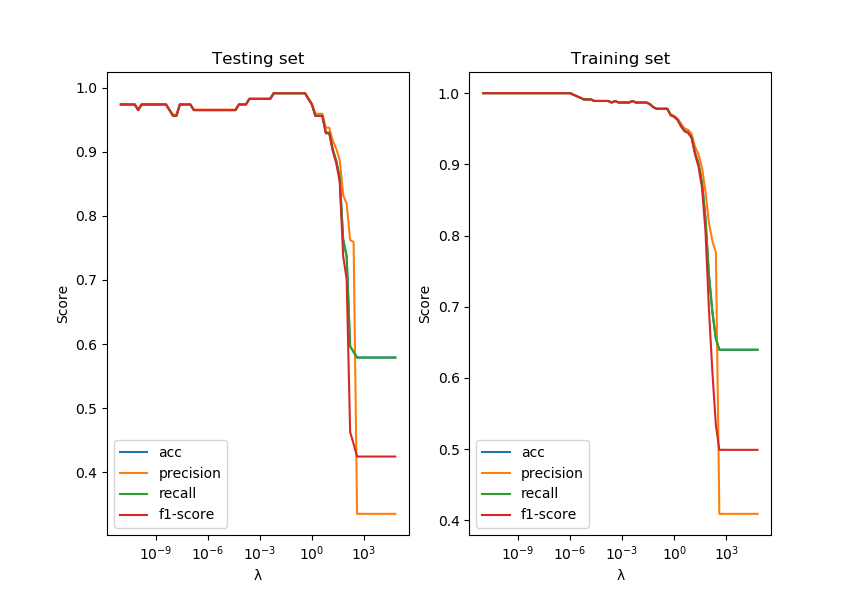
\includegraphics[width=1.2\textwidth]{./fig/fig2.png}
    \cnenfigcaption{低维数据集上效果}{ }
    \label{fig2}
\end{figure}


%%%%%%%%%%%%%%%%%%%%%%%%%%%%%%%%%%%%%%%%%%%%%%%%%%%%%%%
%%% 致谢
%%% 非必选
%%%%%%%%%%%%%%%%%%%%%%%%%%%%%%%%%%%%%%%%%%%%%%%%%%%%%%%
%\Acknowledgements{致谢.}

%%%%%%%%%%%%%%%%%%%%%%%%%%%%%%%%%%%%%%%%%%%%%%%%%%%%%%%
%%% 补充材料说明
%%% 非必选
%%%%%%%%%%%%%%%%%%%%%%%%%%%%%%%%%%%%%%%%%%%%%%%%%%%%%%%
%\Supplements{补充材料.}

%%%%%%%%%%%%%%%%%%%%%%%%%%%%%%%%%%%%%%%%%%%%%%%%%%%%%%%
%%% 参考文献, {}为引用的标签, 数字/字母均可
%%% 文中上标引用: \upcite{1,2}
%%% 文中正常引用: \cite{1,2}
%%%%%%%%%%%%%%%%%%%%%%%%%%%%%%%%%%%%%%%%%%%%%%%%%%%%%%%
\begin{thebibliography}{99}

\bibitem{1} 周志华. "机器学习 (北京: 清华大学出版社) Zhou ZH 2016." Machine Learning (2016).

\bibitem{2} Pedregosa, Fabian, et al. "Scikit-learn: Machine learning in Python." the Journal of machine Learning research 12 (2011): 2825-2830.

\bibitem{3} 拟牛顿法(DFP、BFGS、L-BFGS). https://blog.csdn.net/songbinxu/article/details/79677948

\bibitem{4} Minka, Thomas P. "A comparison of numerical optimizers for 
logistic regression." Unpublished draft (2003): 1-18.

\bibitem{5} Byrd, Richard H., and Jorge Nocedal. "A tool for the analysis of quasi-Newton methods with application to unconstrained minimization." SIAM Journal on Numerical Analysis 26.3 (1989): 727-739.
\end{thebibliography}

\end{document}
%%%%%%%%%%%%%%%%%%%%%%%%%%%%%%%%%%%%%%%%%%%%%%%%%%%%%%%
%%% 附录章节, 自动从A编号, 以\section开始一节
%%% 非必选
%%%%%%%%%%%%%%%%%%%%%%%%%%%%%%%%%%%%%%%%%%%%%%%%%%%%%%%
%\begin{appendix}
%\section{附录}
%附录从这里开始.
%\begin{figure}[H]
%\centering
%%\includegraphics{fig1.eps}
%\cnenfigcaption{附录里的图}{Caption}
%\label{fig1}
%\end{figure}
%\end{appendix}